%!TEX root = mb.tex

\clan{TODO: Reorganize this section, so that it does not have much to do with network processing. Talk about principles primarily in this section, then go into details in firewall section.}

\todo{need to make clear that these enc schemes are not like in CryptDB, that it is not just another CryptDB; only the vision is the same; }% pioneered the vision of extracting core operations and then supporting them. Of course, the core operations are different here

\subsubsection{Range match on encrypted packets} \label{sec:range}

Matching an encrypted value from a packet against an encrypted range is a basic operation for many middleboxes (e.g., firewall). 
For example, it is needed to implement a firewall. 

\mypara{An example} Consider the following firewall rule:

\smallskip
\noindent {\tt block in log quick on \$ext\_if from 10.0.0.0/8  to any
}


\noindent It blocks any traffic from an IP address whose first 8 bits are $10$. This corresponds to an IP address interval of 
[10.0.0.0, 10.255.255.255].
For instance, an incoming packet with IP address 10.1.0.0 will be blocked, whereas a packet with source IP 11.0.0.0 will not be blocked.


The core functionality desired is to be able to encode a set of ranges $[s_1, e_1], \dots, [s_n, e_n]$ into  $[\Enc(s_1)$, $\Enc(e_1)]$, $\dots$, $[\Enc(s_n)$,  $\Enc(e_n)]$, and a value $v$ into $\Enc(v)$, such that anyone (the service provider) having these encodings can determine in which range $v$ lies, if it lies in any interval at all, while not learning the values of $s_1$, $e_1$, $\dots$, $s_n$, $e_n$, and $v$. Hence, we call this scheme {\em range match} scheme. 

In the rest of this section, for concreteness, we explain our scheme by considering $v$, $e_i$ and $s_i$ are source IP addresses, although our scheme can be used for destination IP addresses, ports, etc. Also, since the gateway does the encoding, and the cloud performs the comparisons in our system, we use the same parties when describing our encoding protocol -- although one can envision using it outside of our setting. \todo{does this not contradict itself with tailoring}

\todo{use cloud instead of service provider}

\mypara{Requirements on an encoding scheme}
%
In order for this encryption scheme to fit our systems problem and to do so in a practical way, it must have the following efficiency and security properties. It should:
\begin{enumerate}
\item  {\em be fast}: the performance of the encryption scheme severely affects the throughput of the network,
\item {\em support existing fast packet matching algorithms}: a series of fast matching algorithms are typically used to achieve good performance, such as  various kinds of tries, area-based quadtrees, FIS-trees, or hardware-based algorithms~\cite{packet_classif}.  All of these rely on the ability of the middlebox to compute ``>'' between $v$ and the margins of the intervals, 
hence the encryption scheme should preserve this property. 
\item {\em have as strong security as possible}: The encryption scheme should not leak $v$, $e_1$, $s_1$, $\dots$, $e_n$, $s_n$ to the service provider.
The scheme allows the service provider to compute ``>'' between v and $e_i$ and $s_i$, but ideally it should learn nothing more than this information. In particular, for two values $v_1$ and $v_2$, the service provider should not learn how they compare to the each other (whether $v_1 > v_2$ or not) because it does not need this functionality for range matching. Hence, this scheme is not order preserving, because the service provider does not learn the order of $v_i$-s, and should be more secure than order-preserving schemes.   \label{req:sec}
\item {\em be injective and deterministic}: For integration purposes with NAT, we need to make sure that two different values do not get mapped to the same encryption and the same value gets mapped consistently to the same encryption. \label{req:injective}
\item {\em be format-preserving}: This property is important for performance and ease of adoption. Ideally,  we would like to support firewall hardware {\em unchanged}. Not supporting existing hardware could be slow and requiring deployment of new hardware is challenging for adoption. To use the same hardware, the  encryption should have the same format as the unencrypted value. Namely, it should not be larger or have a different structure than the slot in the packet corresponding to the unencrypted value. 
 \end{enumerate}
 
 \todo{above, the security should be more emphasized and more clear what we seek and get-- range match is what we need not more}
 
 
\todo{agree on parties names in our model}
\todo{is this format-preserving property a more global one?}
\todo{agree if you talk about encoding or encryption scheme -- I prefer encoding and say it is not an encryption scheme}

Unfortunately, there is no encryption scheme that supports all these requirements. The closest scheme to these requirements  is {\em order-preserving encryption}, BCLO~\cite{boldyreva:ope} and mOPE~\cite{popa:mope}. mOPE unfortunately requires that the gateway and the service provider interact for a number of roundtrips (e.g., xxx in our experiments) which is too slow and requires additional setup for this interaction, and violates requirement~\ref{req:sec} or~\ref{req:injective}, and BCLO has weak security (leaking always the top half bits of the values encrypted and the order of IP addresses across different packets, thus violating requirement~\ref{req:sec}), is too slow, and not format-preserving. 

Instead, we designed a new encoding scheme that satisfies all requirements above called {\em range match} scheme. 
The design of the scheme is driven by the systems setting, it is rather a systems technique than an encryption scheme because it leverages the systems setting and uses no cryptographic mathematics or advanced cryptography.  We use cryptography only in order to prove formally the security guarantees of our encoding scheme. Since it is designed for our system setting, its API does not fit into the syntax of an encryption scheme, and so we call it an encoding scheme. 
In addition to being more secure and more fit to this setting than the order-preserving schemes above, our scheme is XXX faster.

\qu{what is more in our favor - to present it as a new encryption scheme that can be understood by a systems audience, or as a new encoding scheme that is mostly a systems technique as above?}


\subsubsection{Our Range Match scheme} 


Recall that we want to design an encoding algorithm using which we can encode intervals  $[\Enc(s_1), \Enc(e_1)]$, $\dots$, $[\Enc(s_n), \Enc(e_n)]$ to be stored at the service provider and then we can encode  $\Enc(v)$, the service provider can determine in which interval $v$ lies, if it lies in any interval at all. 

We explain the scheme based on encoding IP addresses for a firewall and source IP addresses in packets, although the scheme is used in encoding other fields too, as explained in Sec.~\ref{xx}.

The first idea is to encode each endpoint of an interval into a random value while preserving order. For example, we can encode the interval 127.0.0.0/8 and 172.16.0.0/16 into [32.0.0.0, 64.0.0.0] and [96.0.0.0, 128.0.0.0]. This preserves the order of the endpoints of the interval but does not leak the actual intervals. 
The gateway communicates these encoded values to the cloud, and maintains a mapping of interval endpoint  to its encodings, called {\emph interval map}.  The interval map also contains the points $- \infty$ and $+ \infty$, encoded with 0.0.0.0 and 255.255.255.255. 
Note that the number of intervals are small, on the order of xxx, so this results in little storage at the gateway. Moreover, in our algorithm, the gateway will not maintain any state per packet transmitted.

Now when the gateway receives a packet and needs to encrypt an IP address $v$, the gateway first determines what are the two endpoints $v$ falls between -- which could be  endpoints from different intervals. It uses the interval map to determine the encodings of these endpoints. Then, to encode $v$, it can choose a fixed value in this interval, say the middle of the interval. 
For example, if $v$ is 127.0.0.1, a possible encoding is 48.0.0.0, which is the middle of the encoded interval. Given two different packets where we encrypt source IPs, $v_1$ and $v_2$, this strategy maps them to the same encoding; this is great for security because the cloud does not learn the order of $v_1$ and $v_2$ information theoretically -- in fact, the only information it learns is that they are both in the same interval (recall that the endpoints of the interval are also encoded). Thus, this satisfies the security requirement~\ref{req:sec} above, and makes our scheme more secure than order-preserving encryption schemes (which leak order across all IP addresses encoded).

However, the injective requirement~\ref{req:injective} is violated: two IP addresses are assigned the same value. 
To fix this, the idea is for the gateway to assign to $v$ a random value in the corresponding encoded interval, and the next time it encodes $v$, it should assign the same value. 
Still, we need to fix two issues: make sure that the gateway knows to map $v$ to the same encoding the next time it encode its, and that  the probability of mapping two different values to the same encoding if negligibly low.
One idea is to store a table at the gateway that recalls the values $v$ encoded  so far and the encodings to which were mapped, to prevent duplicates. However, this would require significant state at the gateway. Instead, the idea is to use a pseudorandom function $\prf$ seeded in $k$. This function has the property that it maps a value $v$ to a random value in a deterministic way.  Let $[\low, \high]$ be the interval of {\em encodings} that correspond to $v$. 
Then, the encoding of $v$ is computed as:
\[ \enc(v) = \low + \prf_k(v)\ \mod\ (\high - \low), \] 
which is  a random value in the interval $[\low, \high]$. This function is deterministic.
For example, 127.0.0.1 could be encoded into 62.211.52.17. 
To have a very low chance of collisions, we ensure that each interval of encodings is as large as possible: hence, we distribute the evenly the intervals to be encoded over the whole IP space from 0.0.0.0 to 255.255.255.255 -- without a priori knowledge on what values $v$ will be encoded, the uniform distribution is the best strategy. We show in \S\ref{sec:eval} XXX that the chance of collisions becomes very small considering a generous upper bound on the number of intervals in firewall rules today.


The last issue to address is what happens when firewall rules get updated, and say, a new interval gets inserted. 
Since we tried to spread out the encodings of the intervals evenly in the IP space, there is no room for a new interval. We can 
readjust all the encodings of these intervals to make space for the new interval. However, this would require the firewall hardware to reconfigure fully which is slow. Ideally, we would only reconfigure the firewall hardware incrementally, for the new interval. For this, we build on the idea from mOPE~\cite{popa:mope} and store the intervals at the gateway in a balanced scapegoat tree as in Fig.~\ref{fig:tree} -- our use of the tree is different from mOPE~\cite{popa:mope} as discussed in \S XXX. \qu{even bother to discuss differences when we have clearly better performance?} The scapegoat tree gives us the property that when a new interval is inserted, a small number of interval encodings are changed, logarithmic amortized worst case. Each node in the tree is now encoded similarly to before: the root gets the middle of the IP range,  the left node gets the middle of the IP space to the left of the middle, and so on, as in Fig.~\ref{fig:tree}.  Note that, since the tree is balanced, it maintains our desire of having intervals of encodings roughly even in size (the smallest and largest are guaranteed to be within a factor of XXX of each other).

\begin{figure}
  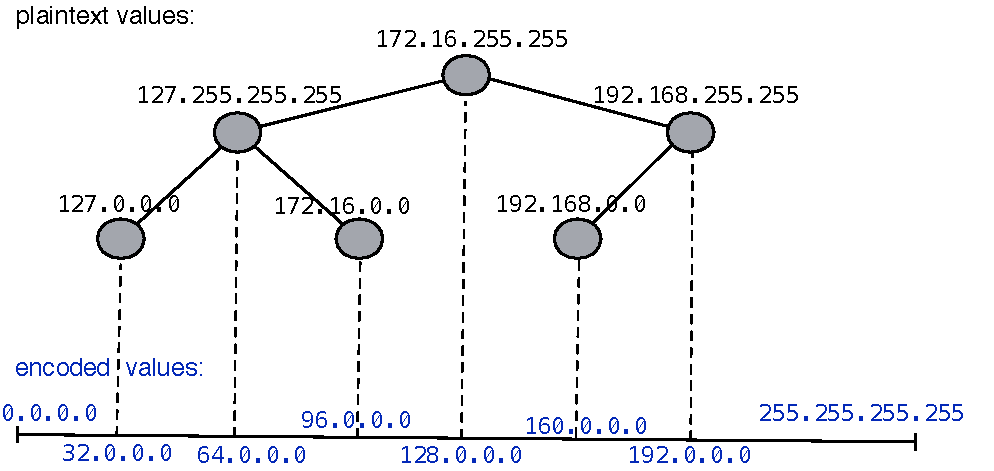
\includegraphics[width=3.45in]{fig/tree}
  \caption{\label{fig:tree} Range match tree. The values of nodes in the tree are the unencrypted IP addresses, and the blue values on the horizontal axis are their encodings. }
\end{figure}



\qu{what happens to collisions w.r.t. port numbers?}
\todo{need to introduce the key k somewhere}

We now explain concretely the API and the implementation of the scheme. 

\subsubsection{Gateway API}

The gateway can use the following functions. 

EncodeRanges encodes the initial ranges. Note that some ranges could consist of
one point only, namely $s = e$. 

% TO CUT TO REDUCE: put all these algorithms into one box

\begin{framed}
\begin{algorithmic}[1]

\Procedure{EncodeRanges}{[$s_1$, $e_1$], $\dots$, [$s_n$, $e_n$]}
  \State Build scapegoat tree on the values 
              $\{s_1, \dots, s_n\}$ 
              $\cup$ $\{e_1, \dots, e_n\}$ 
              $\cup$ $\{-\infty, \infty\}$.
  \State Assign an encoding $\enc(x)$ to each node $x$ in the tree:
  \begin{itemize}
  \item the root gets the middle of the IP range, $e$, 
  \item the left node to the root gets the middle of the range left of $e$ ($e/2$),
  \item the right node gets the middle of the range
  to the right of $e$ ($3e/2$), and so on.
  \end{itemize}

  \State \Return{[$\enc(s_1)$, $\enc(e_1)$], $\dots$, [$\enc(s_n)$, $\enc(e_n)$]}
\EndProcedure

\end{algorithmic}
\end{framed}

EncodeValue encodes the values to be matched against ranges.

\begin{framed}
\begin{algorithmic}[1]

\Procedure{EncodeValue}{$v$}
  \State Search the tree for $v$ to identify the tightest enclosing interval [$p_1$, $p_2$]. 
  \State Let $\low$ and $\high$ be the encodings of $p_1$ and $p_2$. 
  \State Compute $\enc(v) = \low + \prf_k(v)\ \mod\ (\high - \low)$
   \State \Return{$\enc(v)$}
\EndProcedure

\end{algorithmic}
\end{framed}

Note that the search for $p_1$ and $p_2$ is fast, logarithmic time, due to the fact that the 
scapegoat tree is a balanced search tree. 

We now present AddRange and DeleteRange which update the state at the firewall with new rules. 

\begin{framed}
\begin{algorithmic}[1]

\Procedure{AddRange}{$[s, e]$}
  \State Insert $s$ and $e$ in the scapegoat tree. If $s=e$, insert the value only once.
  %	
  \State Initialize $L$ to be the empty list.
  \If{tree needs to be rebalanced}
  	\State Record which nodes change position in the tree during rebalancing, together with 
	their old and new encodings. Namely, record	\[L = \{ \en_1 \leftarrow \en^*_1, \dots, \en_m \rightarrow \en^*_m\},\] where $m$ is the number of nodes who changed position in the tree, and $\en_i$ and $\en^*_i$ are the old and new encoding of the $i$-th node that changed position. 
  \EndIf
  \State Compute  $\enc(s)$ and $\enc(e)$, the encodings of $s$ and $e$, as in EncodeRanges.
   \State \Return{$[\enc(s), \enc(e)], L$}
\EndProcedure

\end{algorithmic}
\end{framed}


Since we are using a scapegoat tree, the number of nodes that change position during rebalancing is amortized worst case $O(\log n)$ where $n$ is the total number of nodes in the scapegoat tree. 

DeleteRange is similar, except that the only result is the list $L$ of changes. 

\subsubsection{Cloud API}

The cloud can run ``$\ge$'' and "$\le$" between any encoded value $\enc(v)$ and encoded enpoint $\enc(s)$ and $\enc(e)$, and obtain a correct answer. Computing $\enc(v_1) < \enc(v_2)$ is meaningless, and returns a random value.


 
\todo{somewhere explain its security with an example -- significantly more secure than enc schemes used in CryptDB, etc}


 






% make differences from mope more clear 

\todo{must emphasize provable guarantees and point to a tech report or something with proofs}
\todo{I think you need to express the security of the scheme again somewhere}


\todo{consistency of encoding vs encryption}




% PROTOCOL

% the gateway encrypts teh IP has to be clear

% Here somewhere we need to discuss that there is one encryption scheme adn then there is how we use it for ports and other ip addresses.

% in the firewall protocol describe how hardware does not change 

% can use the same processing 
